%
% File naaclhlt2016.tex
%

\documentclass[11pt,letterpaper]{article}
\usepackage{naaclhlt2016}
\usepackage{times}
\usepackage{latexsym}
\usepackage{hyperref}
\usepackage{url}
\usepackage{graphicx}
\naaclfinalcopy % Uncomment this line for the final submission
%\def\naaclpaperid{***} %  Enter the naacl Paper ID here

% To expand the titlebox for more authors, uncomment
% below and set accordingly.
\addtolength\titlebox{.5in}    

\newcommand\BibTeX{B{\sc ib}\TeX}

%
\title{Menu Price Prediction using Neural Networks}

% Author information can be set in various styles:
% For several authors from the same institution:
% \author{Author 1 \and ... \and Author n \\
%         Address line \\ ... \\ Address line}
% if the names do not fit well on one line use
%         Author 1 \\ {\bf Author 2} \\ ... \\ {\bf Author n} \\
% For authors from different institutions:
% \author{Author 1 \\ Address line \\  ... \\ Address line
%         \And  ... \And
%         Author n \\ Address line \\ ... \\ Address line}
% To start a seperate ``row'' of authors use \AND, as in
% \author{Author 1 \\ Address line \\  ... \\ Address line
%         \AND
%         Author 2 \\ Address line \\ ... \\ Address line \And
%         Author 3 \\ Address line \\ ... \\ Address line}
% If the title and author information does not fit in the area allocated,
% place \setlength\titlebox{<new height>} right after
% at the top, where <new height> can be something larger than 2.25in
\author{Michele Ceru \\
	    Center for Data Science\\
		New York University\\
	    {\tt mc3784@nyu.edu}
	  \And
	Luisa Quispe Ortiz\\
  	Center for Data Science \\
  	New York University\\
  {\tt lqo202@nyu.edu}}

\date{}

\begin{document}

\maketitle

\begin{abstract}
Culture diversity and socioeconomical groups strenghten are marked by the way language is used in each of them.
Many studies have shown that there is a relation between how a restaurant describes itself and price a restaurant charge (or the price range it has), based on the previous statement. Therefore, it may be possible to find use menu's description to predict the price of a dish. We aim  to perform this task taking advantage of tools such as word embeddings and neural networks, that we believe will aide and facilitate the objective.
\end{abstract}

\section{Introduction}

New York is known as being a city that has influence of several cultures so it's logical that its cuisine reflects that too. Across all the city it is possible to find chinese, italian, mexican and many more kitchen’s of the world having a myriad of plates and prices.

Many factors influence the price, from external sources such as inflation, availability, critic’s reviews and even customer opinions \cite{jurafsky2014language}.

Each restaurant knows their target customer, hence all the business is focused on it including the menus. This implies a relation between socioeconomic class and language \cite{freedman2011authenticity}, which implies also Bordieu's distinction \cite{jurafsky2016bordieu}. Therefore, there is evidence of a relation between how a restaurant describes its plates and how much it charges. Would it be possible to predict the price of a dish given its description?

There are some previous works that are related to the mentioned task, some of them from a economics, culinary approach or a linguistics point of view. The objective varies according to the approach taken. For example, in economics it is important to see the impacts of reviews on sells, while in culinary and hospilatity the objective is to analyze language used in the menus to mainly make recommendations for writing \cite{chahuneau2012word}.

Although the variety, some handful insights were found such as in \cite{chahuneau2012word,jurafsky2014language,jurafsky2016bordieu}: 5-stars restaurants tend to use more fancy words and borrow expressions from other languages making the description larger but succinct, while cheaper restaurants have a wider variety of food and tends to use just a small phrase to describe its plates and focus on adjectives and filler words. 

None of the previous literature, however, used distributed word representations and neural networks to predict the menu's price per item using just text. Using word representations will aide to understand the underlying semantic relation between words \cite{mikolov2013efficient} in the culinary aspect. And training using neural networks will bring us the possibility of capturing non-linear relationships \cite{beale1990neural} between the embeddings and the target variable price , even more if we consider the dynamics of word order as in recurrent neural networks (LSTM or GRU). We believe that it's possible to confirm some conclusion other studies have had, besides reaching an improvement of the evaluation metric due to the use of the mentioned deep learning tools.


\section{Prior Literature}

As stated in \cite{chahuneau2012word}, most of the previous works are in the linguistics, hospitality research and economics fields. Each of them gives a slightly different approach, a few focusing in predicting price range of a restaurant and others in the analysis of the linguistic implications of the menu. However, it's good to have a starting point.

Socieconomic groups are defined by the way they use the language, this is widely known and used by politicians. In \cite{freedman2011authenticity}, the authors claim that the previous phrase is true, even more, they assert that food is a "robust marker of group identity" too. They show that prices affect the language in food advertising, specifically in potato chip bags. A similar study, this time experimental was done in \cite{mccall2008effects} but to see implications of text complexity on perceptions of quality and purchase intentions. The view was more psychological, and they proved that longer, more descriptive menu lines usually made the consumer think it was expensive.

There has been also works in prediction using text, such as the one described in \cite{archak2011deriving} where they analyze the impact of reviews on product sales, a marketing and economics point of view. They focus on a couple of products and identify "beliefs" a customer has in a product's feature, not considering a polarized review (positive or negative based on the rating). This has not been the only prediction task using text that can be found, some examples are predicting risk in financial markets or using reviews to predict movies profitability \cite{joshi2010movie}, to other several economic tasks. 

In the field of culinary and hospitality research, there are many manuals that have recommendations for writing menu descriptions, according to \cite{chahuneau2012word} and \cite{jurafsky2014language}, such as \cite{kasavana1990menu} . Actually is interesting to notice that by conducting an experiment in a small cafeteria \cite{wansink2005descriptive} showed that the menu description does affect the customer's behavior and perception.

The logic that menu's descriptions produce change considering the restaurant's market niche (public they are directed to), and the fact that this follows linguistic socieconomical differentiation, is mentioned and explained in the first chapter of \cite{jurafsky2014language}, where he cites a some works and their main implications in the relationship between prices and descriptions, besides giving his own perceptions. Jurafsky assures that expensive restaurants' menus tend to use "native" words borrowed from other languages such as french, italian, spanish; they use fancy words in long descriptions and they focus more in the detail of the description and avoid using filler words. On the other hand, common cheaper restaurants have a wider variety of plates, for, they try to sell them by describing in a simple and shorter way using a lot of filler words ("real cream cheese", "home-baked cookies"). 

Our main source is  \cite{chahuneau2012word}, as one its goals is to predict the price and how it is influenced by the use of language. The article uses menu descriptions from main cities across the U.S. as well as some descriptive features extracted from Yelp reviews (flag variables of wi-fi, parking, delivery, etc). Their analysis is mainly linguistical, as they wish to know how each word or change of word affects the price, using regression tools.

In a more recent background, a study  \cite{jurafsky2016bordieu} focuses on studying the reflections of Bourdieu's distinction, which happens to consider that there are deep associations linking food culture with social class and other aspects of identity, using the language of food. They split their study in 4 aspects, that define the relation between food and social culture aiming to predict the price range a restaurant belongs to. Using Yelp reviews they conclude that words used in menu descriptions reflect the many aspects of Bourdieu's distinction, therefore these help determine the price range. In general terms, the insights found are mainly the ones mentioned in the previous paragraphs with a couple of new findings (e.g. adjectives are used mostly in cheaper backgrounds), so the study is kind of confirmatory.

Finally, a more studied related field involves sentiment analysis using reviews, there are plenty of state-of-the-art literature. Some use a more traditional approach such as in \cite{jurafsky2014narrative}, while others start using deep learning to get better results \cite{tang2015document}.

\section{Data}
To gather the information required by the project, we considered previous works and decided to crawl AllMenus.com (\url{www.allmenus.com}). Initially we only got New York City menus, but to ensure consistency in our results by having a larger sample, we decided to include San Francisco. We ended up with 467,669 NY menu descriptions and 200,020 from SF. For us, each of these rows is a observational instance corresponding to a menu item. So, the features captured were: restaurant name,  section of the menu, subsection of the menu, dish name, dish price and description, from which we will take the price as our target and the dish name and description as our input text.

Before moving on the modeling task, we made a quick analysis of our information in order to detect any anomaly.  The first we could find is that only 99 observations had null price which we set to zero price (and later erased), the rest was encoded in different ways but it was possible to obtain the price value of the plate. 

Then, we wanted to see the distributions per city, and whether there was significant difference that pointed us to do separately analysis. The mean price of SF is of \$9.77, one more dollar than the mean of NYC, a similar relation was found in the medians as NYC's was of \$6.99 against \$7.99 in SF. Despite this, by looking at the normalized (standardized) distributions in Figure \ref{fig:price_dist} it was possible to see that both seem alike, highly skewed. 

   \begin{figure}[thpb]
      \centering
      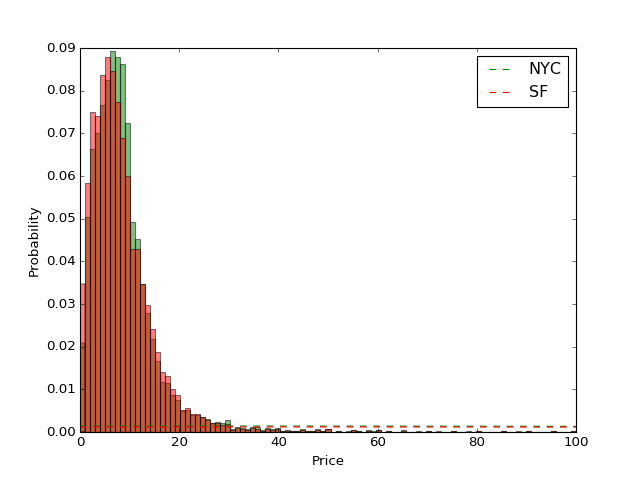
\includegraphics[width=6cm, height=4cm]{dist_sf_nyc_prices}
      \caption{Distribution of the prices in NYC and SF}
      \label{fig:price_dist}
   \end{figure}

This gave us evidence to keep on analyzing all the dataset together. 

In the text, we made a tokenizer that deleted some punctuation signs and that lower case all the input text.

For all our runs, the whole data set of restaurants item's price was split into training(80\%), validation (10\%) and testing(10\%) set randomly, considering that the proportion of observations per city will be the same due to randomness. 

\section{Modeling Framework}
\subsection{Some definitions}
Before explaining our protocol, we give some brief definitions about the tools that will be used.
\paragraph{Word Embedding}
Distributed representation of words are widely used nowadays, they are just ubiquitous to most NLP tasks, as they provide semantic relation between words \cite{hill2016learning}.  A good example is the known neural embedding \textbf{Word2Vec} result of an Google's experiment which trains words against other words that neighbor them in the input corpus. Their approach based on two techniques, the first predicts the word that is in the middle based on the 4 surrounding neighbors which is known as Continuous Bag of Words. The second model is actually the reverse process, to predict the words around a specific one known, called Skip-gram \cite{mikolov2013distributed,mikolov2013efficient}. 

For some experiments, we'll use the pretrained Word2Vec inputs, as they are available online (\url{https://deeplearning4j.org/word2vec}). There are 3 million vectorized words which have a dimension of 300.

\paragraph{Neural Networks}
Neural networks (deep learning) have started to be used in NLP for a while now. Most of them are used in tasks such as sentiment analysis, POS tagging, and machine translation tasks \cite{cho2015natural}. 

One of the most used neural networks is the recurrent neural networks Long Short Term Memory and Gated Recurrent Unit \cite{cho2015natural} as they don't suffer from vanishing or exploding gradient problems. A huge advantage of GRU and LSTM is that they capture the sentence sequence dynamics, therefore it is possible to get more insights (semantically and syntactically) of the whole text \cite{gers2000learning,cho2014learning,cho2015natural}.

There's some literature that suggest working schemes for continuous targets such as in \cite{regneural1991} which uses a statistical framework. Based on material seen in class and on \cite{cho2015natural} we find that by changing the loss function, it is possible to focus in a continuous target. We'll use both, categorical an continuous targets in the neural networks to predict price of a restaurant menu's item.

\subsection{Protocols Proposed}
As it has been stated, the proposed work just considers text as input (item's descriptions and names) to predict a target which is the price. We planned to launch some experiments considering the embedding type, the type of neural network and the type of target.
\begin{table}[ht!]
\centering
\caption{Experiment setup}
\label{table:experiment-setup}
\scalebox{0.8} 
{\begin{tabular}{|l|l|l|}
\hline
\textbf{Target type} & \textbf{Embedding Type} & \textbf{Neural Nework} \\ \hline \hline
Class & Self-learned & MLP \\ \hline
Class & Self-learned & LSTM \\ \hline
Class & W2V fixed & MLP \\ \hline
Class & W2V fixed & LSTM \\ \hline
Class & W2V initial & MLP \\ \hline
Class & W2V initial & LSTM \\ \hline
Continuous & Self-learned & MLP \\ \hline
Continuous & Self-learned & LSTM \\ \hline
Continuous & W2V fixed & MLP \\ \hline
Continuous & W2V fixed & LSTM \\ \hline
Continuous & W2V initial & MLP \\ \hline
Continuous & W2V initial & LSTM \\ \hline \hline
\end{tabular}}
\end{table}

Regarding the embedding, it was possible to set the initial embedding to random numbers, so that it would be another parameter to estimate. Another option was to make the embedding not trainable so it would be a fixed pre-trained matrix. A third option consisted in a mix of the previous: instead of starting from a random point, the embedding matrix could be trained starting from a pre-trained matrix and learned through the optimization process. We decided to used pre-trained Word2Vec embeddings(W2V) in the cases pre-trained matrices were needed. 

Another option in modeling was to take into account the order of the words, which is usually captured by a recurrent neural network: a LSTM or GRU. Since we wanted to know if order mattered, we decided to launch a  Multilayer Perceptron (MLP) and a LSTM based model for the experiments. 

Finally, we had to decided how was the price target going to be predicted. As most of the literature focuses in range predictions, we choose that path first: priced were group in 10 labels cuts were \$5 dollars. This selection was made in order to try capture the tail of the distribution, given that if percentiles were chosen steps between groups may be too short. 

To give another point of view and to made our experiments comparable, we decided to use a continuous target by setting the loss function to a squared loss.

Our final setup can be seen in Table \ref{table:experiment-setup}. 

\subsection{Model Configuration}

All the models are believed to have the default configuration showed in Table \ref{table:def-config}, otherwise the change will be explicitly mentioned.
\begin{table}[ht!]
\centering
\caption{Default Configuration}
\label{table:def-config}
\scalebox{0.8} 
{\begin{tabular}{|l|l|}
\hline
\textbf{Configuration Variable} & \textbf{Value} \\ \hline \hline
BATCH\_SIZE & 64 \\ 
CHECKPOINT\_EVERY & 200 \\ 
DROPOUT\_KEEP\_PROB & 1 \\ 
EMBEDDING\_DIM & 300 \\ 
EVALUATE\_EVERY & 50 \\ 
INIT\_SCALE & 0.1 \\ 
L2\_REG\_LAMBDA & 0 \\ 
MAX\_GRAD\_NORM & 5 \\ 
NUM\_EPOCHS & 10 \\ \hline \hline
\end{tabular}}
\end{table}

The optimizer used depended on the model, for MLP Adam Optimizer was used, with a learning rate of 0.003. For the RNN LSTM a Gradient Descent was used using an initial learning rate of 1, and then a decay of 0.5 if no improvement was found.  Some experiments though considered for all the neural networks an Adam Optimizer, again if so it will be said explicitly. 

Besides all the mentioned details, specifically for the LSTM cell, we considered a mean of all the output states ($h_t$) similar to what is done in .

\subsection{Training and Model Selection}
We trained some models considering the 10 epochs, but most of them were trained with a 4 step early stopping, similar to what's suggested in \cite{cho2015natural}. 

Our metric to evaluate the early stop was based on the loss function. If in 4 evaluation periods the loss was increasing it meant that the model reached a local optima. 

All of our runs were done in a HPC server requesting around 32GB of RAM and 1 GPU unit, and depending on the experiment it could take from an hour to 36 hours to finish. 

\subsection{Evaluation}
Depending of the whether the model was continuous or class it had different loss functions. Therefore, for the class we used accuracy as the main indicator to see how well the model was performing. The loss in this case was set to use a cross entropy (having behind it a 10 class categorical distribution). 
For the continuous model our performance metric was the mean squared error and the mean absolute error, using a mean squared L2-norm as stated in \cite{cho2015natural}.

Furthermore, in order to have more insights on what our model was driven by, we decided to look at the resulting embeddings and see how words affect the price prediction. For the primer, using t-SNE (PCA component) to reduce dimensionality to 2D helped us to plot the embedding. Also, for the latter, we adapted a script to predict interactively prices, this will help us to understand the influence of words. The objective here was to see if our models capture the relations explained in all the state-of-the art literature mentioned in part 2: expensive restaurants characterize for using foreign words, making long descriptions but not using filler words nor adjective while cheaper restaurants tend to focus more in describe provenance and use a lot of filler words ("real", "over",etc). 

\section{Results}
Results running all the epochs are displayed in .
They show that there is a gain in running the 10 epochs, but it may not be worth to do it as the results do not increase drastically. 


On the other hand, we had a bunch of models to select from each of protocol we decided to test since randomnes of the batches affected of all them. The best among all our results per category are shown in Table \ref{table:summary-results}. 
\begin{table*}[ht!]
\centering
\caption{Best results by protocol}
\label{table:summary-results}
\scalebox{0.8} 
{\begin{tabular}{|l|l|l|l|l|l|l|l|}
\hline
\textbf{Target type} & \textbf{Embedding Type} & \textbf{Neural Network} & \textbf{Loss Type} & \textbf{Training Loss} & \textbf{Dev. Loss} & \textbf{Test Loss} & \textbf{Indicator} \\ \hline\hline
Class & Self-learned & MLP & Cross-entropy &  &  &  &  \\ \hline
Class & Self-learned & LSTM & Cross-entropy &  &  &  &  \\ \hline
Class & W2V fixed & MLP & Cross-entropy &  &  &  &  \\ \hline
Class & W2V fixed & LSTM & Cross-entropy &  &  &  &  \\ \hline
Class & W2V initial & MLP & Cross-entropy &  &  &  &  \\ \hline
Class & W2V initial & LSTM & Cross-entropy &  &  &  &  \\ \hline
Continuous & Self-learned & MLP & Squared &  &  &  &  \\ \hline
Continuous & Self-learned & LSTM & Squared &  &  &  &  \\ \hline
Continuous & W2V fixed & MLP & Squared &  &  &  &  \\ \hline
Continuous & W2V fixed & LSTM & Squared &  &  &  &  \\ \hline
Continuous & W2V initial & MLP & Squared &  &  &  &  \\ \hline
Continuous & W2V initial & LSTM & Squared &  &  &  &  \\ \hline \hline
\end{tabular}}
\end{table*}

As part of the evaluation, in order to understand more about the model, we chose top 100 words in frequency of a learned embedding. The chosen model was , whose project embedding is 2D is displayed in . 

Finally, we evaluated a couple of models with our interactive prediction section. We tested some phrases found on \cite{jurafsky2014language} to see how our models reacted.  The results of this evaluation are displayed in table



\section{Analysis}
\section{Conclusions}

\paragraph{Limitations}

\paragraph{Future Work}
We used word embedding as word representation to capture the syntactic relation between words. However, it is possible to use sentence embeddings to see if these capture more and therefore brings a better model \cite{}

\section*{Acknowledgments}
We'd like to thank Prof. Bowman for allowing us to the explore relationship between text in food descriptions and prices using neural networks, and for his advice throughout the project.
\section*{Collaboration Statement}

\bibliography{naaclhlt2016}
\bibliographystyle{naaclhlt2016}



\end{document}